\documentclass[12pt]{article}
\usepackage{amsmath, amsfonts, amssymb, amsthm}
\usepackage[margin=1in]{geometry}
\usepackage{asymptote}
\usepackage{lastpage}
\usepackage{fancyhdr}
\usepackage{parskip}
\usepackage{ulem}
\pagestyle{fancy}
\headheight 25pt
\lhead{Team 24}
\chead{Citadel Datathon}
\rhead{February 23, 2019}
\cfoot{Page \thepage\ of \pageref{LastPage}}


\title{Citadel Datathon Report}
\author{Team 24\\\\Jesse Zhong, Kevin Feng, and Qing Huang}
\date{February 23, 2019}
\begin{document}
\maketitle 
\newpage
\section{Executive Summary}

\subsection{Background and Question}
With the world growing increasingly alarmed at the impact that emissions have on the global environment and the mounting evidence of climate change, countries have started committing to decreasing carbon emissions and finding ways to shift to cleaner energy. Within the United States, many states have shifted from using coal or natural gas to renewable sources such as hydroelectric, solar, and wind energy, and the global renewable energy market is expected to reach record high market demand in the decade to come. 

However, one of the key issues is whether it is profitable for businesses to create power plants that rely renewable resources, and whether or not the current supply and demand make such businesses viable. Thus, our topic question is: \textbf{What can we discover about the market potential of renewable resources within the United States?}

\subsection{Process and Findings}
Using the given data tables, we examined various factors that affect market potential for three forms of renewable energy, hydroelectric, solar, and wind, such as market competition, energy generation and consumption, and overall population. 

Using the $power\_plants.csv$ data, we plotted analyzed the locations of power plants in the United States based on the type of renewable resource they implemented, and found that market competition mainly lies along the East and West coasts, especially in states such as California, North Carolina, and Massachusetts. Furthermore, there is a distinct lack of power plants in the Midwest, so businesses that choose to invest there would find little to no competition. 

We also used data from the $seds.csv$ to analyze the generation and consumption of each type of energy within each state, finding that consumption, in most cases, outpaced generation. But within some states, there was data showing that consumption of a certain type of energy had been greater than its generation for many years, showing great potential for businesses to enter the market.

\section{Technical Analysis}
We first mapped the locations of various power plants utilizing the three main forms of renewable energy across the United States. In the figures below, the size of the plotted points represent the amount of energy generated. 

\begin{figure}[!htbp]
\centering
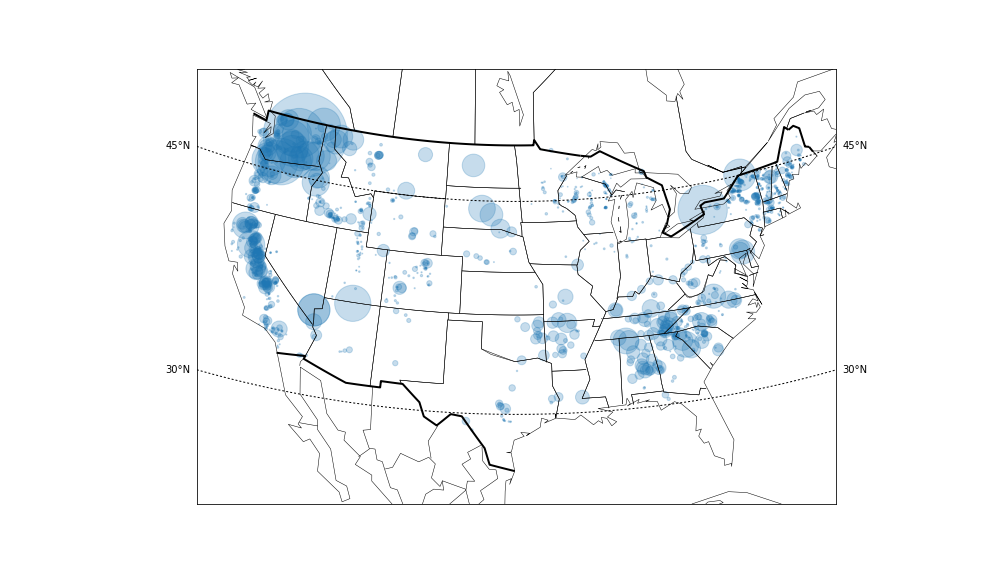
\includegraphics[width=1\textwidth]{hydro.png}
\caption{Hydroelectric Power Plant Map}
\end{figure}

\begin{figure}[!htbp]
\centering
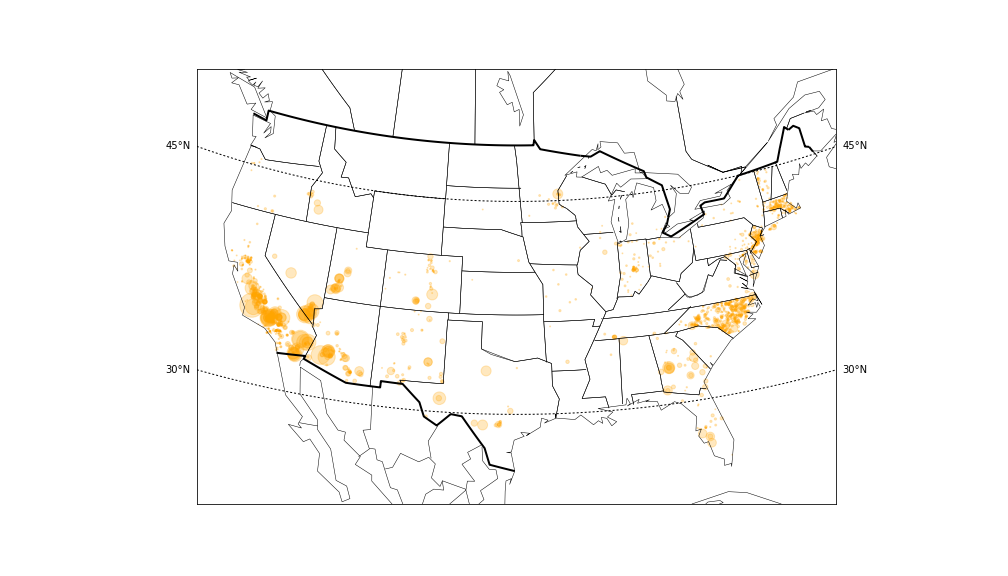
\includegraphics[width=1\textwidth]{solar.png}
\caption{Solar Power Plant Map}
\end{figure}

\begin{figure}[!htbp]
\centering
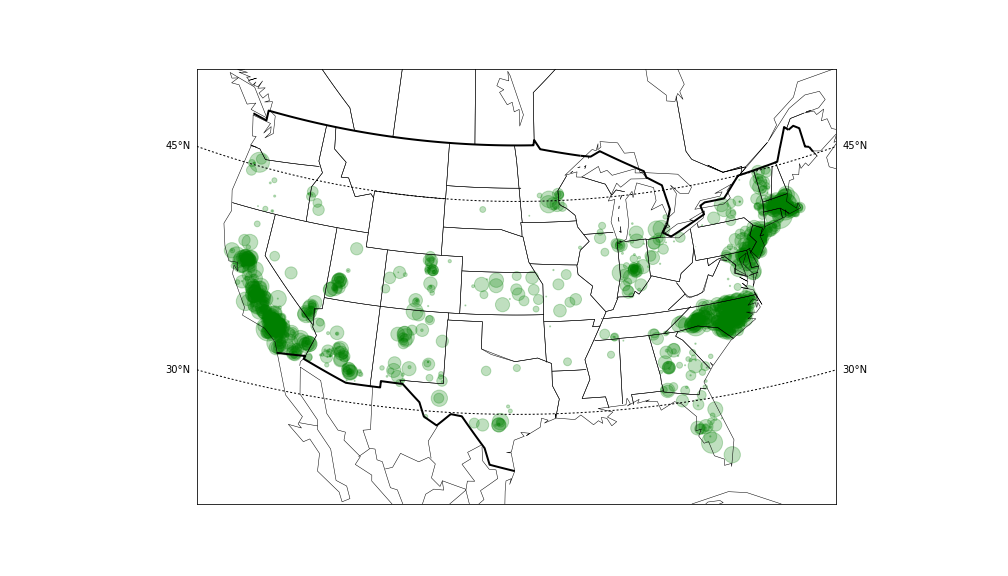
\includegraphics[width=1\textwidth]{wind.png}
\caption{Wind Power Plant Map}
\end{figure}

\newpage 

Some interesting observations are how solar and wind power plants are in very similar locations, and how they are generally located in high-population cities. North Carolina is a clear outlier in the data, having a large concentration of solar and especially wind power plants, which perhaps relates to state legislature for cleaner energy. 

For water power plants, we see that they are more spread out and slightly further inland than the solar and wind power plants, which perhaps indicates their close proximity to large rivers that are close to the coastline.

\newpage
\begin{figure}[!htbp]
\centering
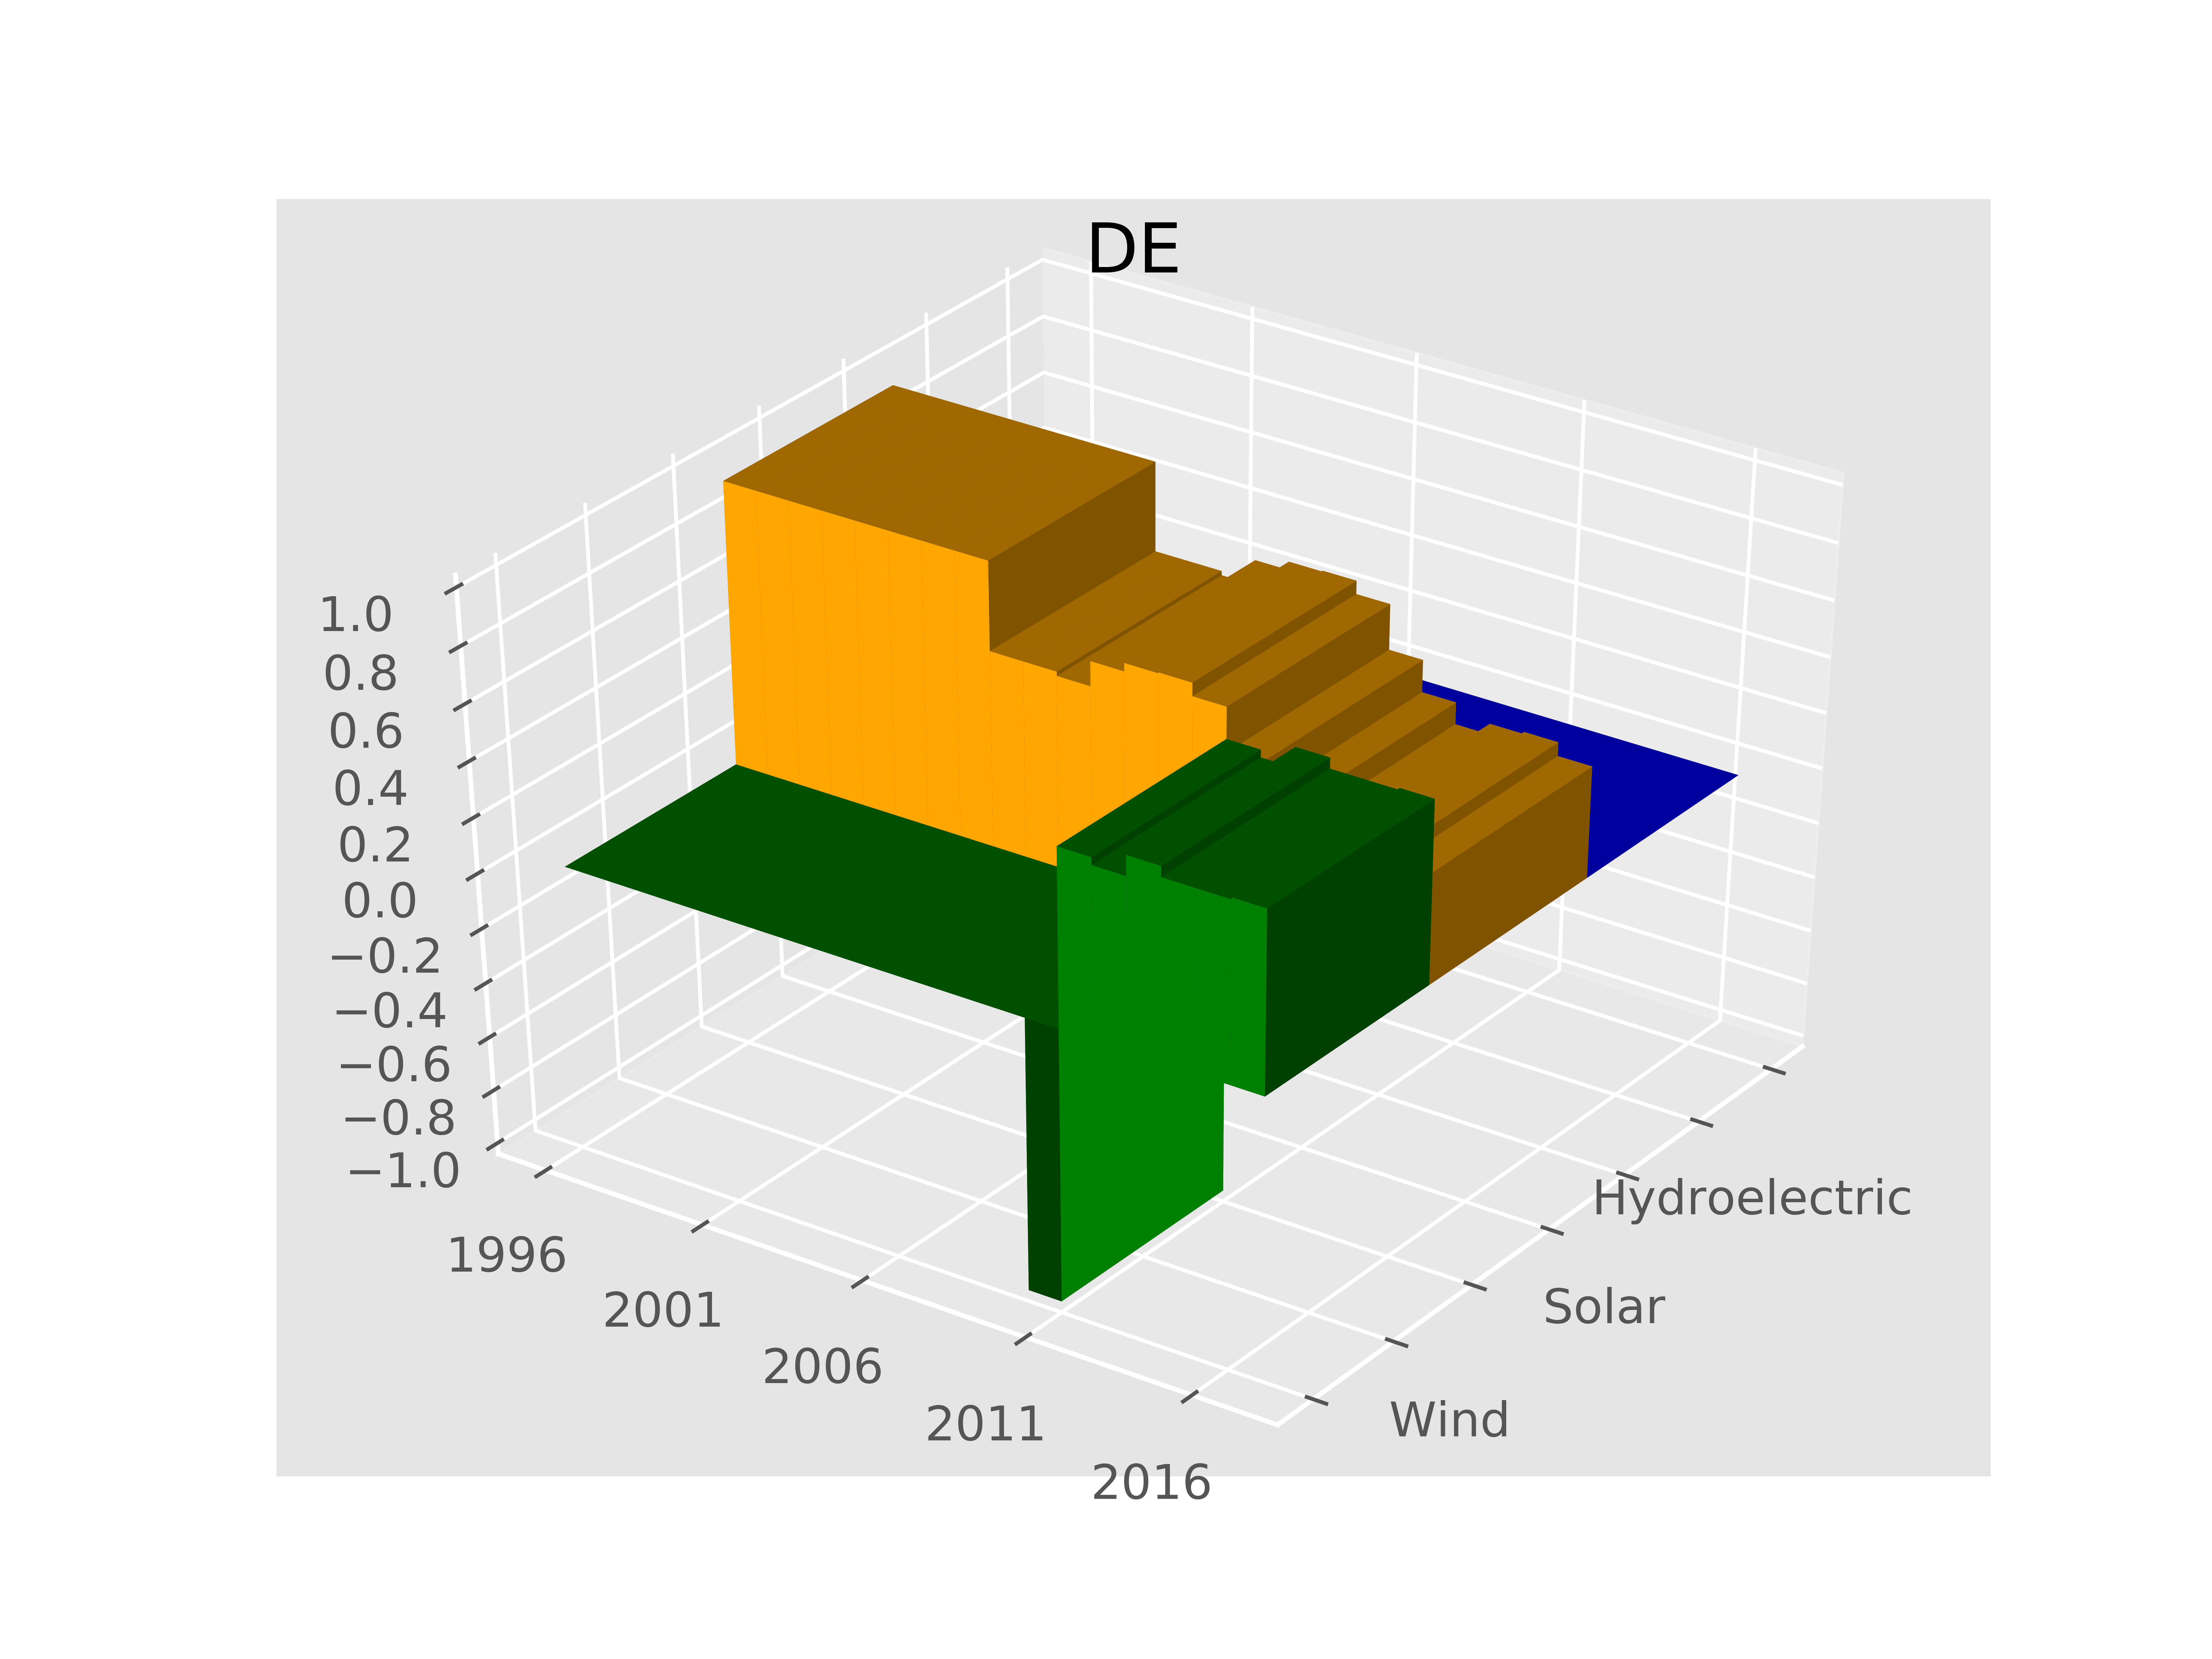
\includegraphics[width=0.85\textwidth]{DE.png}
\end{figure}


\begin{figure}[!htbp]
\centering
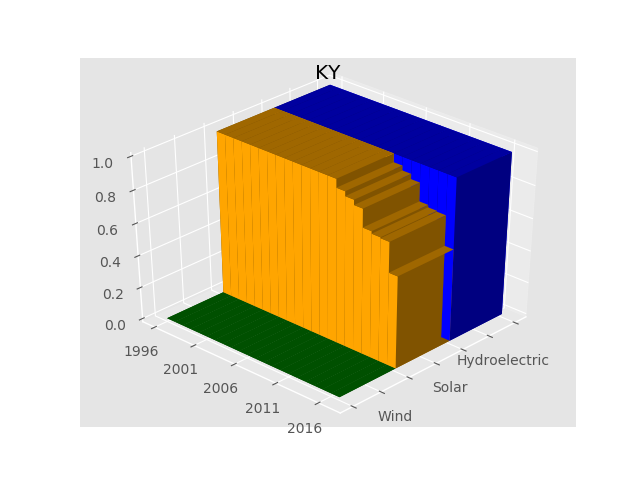
\includegraphics[width=0.85\textwidth]{KY.png}
\end{figure}

\begin{figure}[!htbp]
\centering
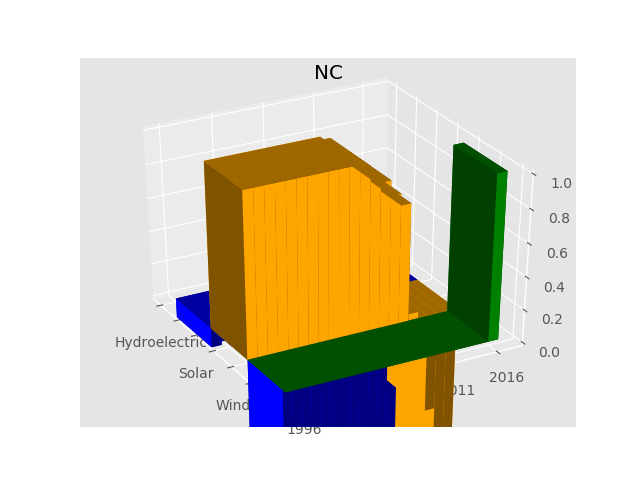
\includegraphics[width=0.85\textwidth]{NC.png}
\end{figure}

\begin{figure}[!htbp]
\centering
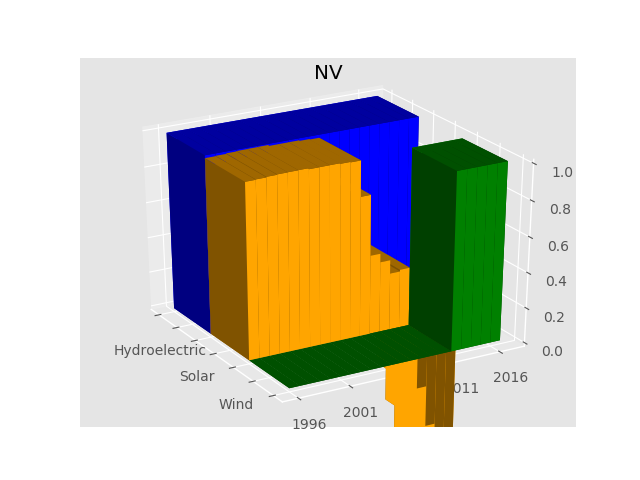
\includegraphics[width=0.85\textwidth]{NV.png}
\end{figure}

\begin{figure}[!htbp]
\centering
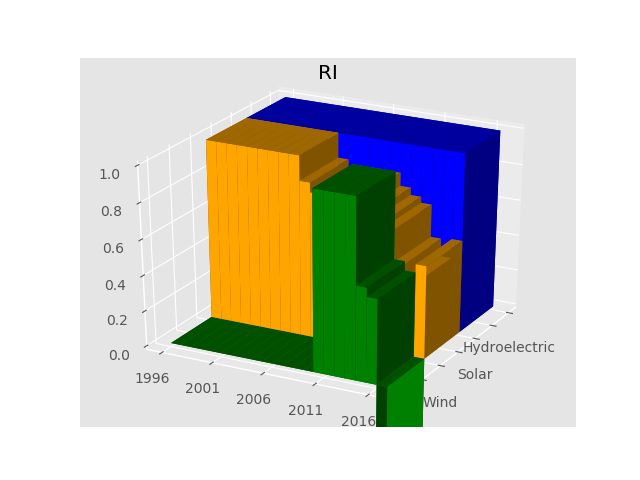
\includegraphics[width=0.85\textwidth]{RI.png}
\end{figure}

\begin{figure}[!htbp]
\centering
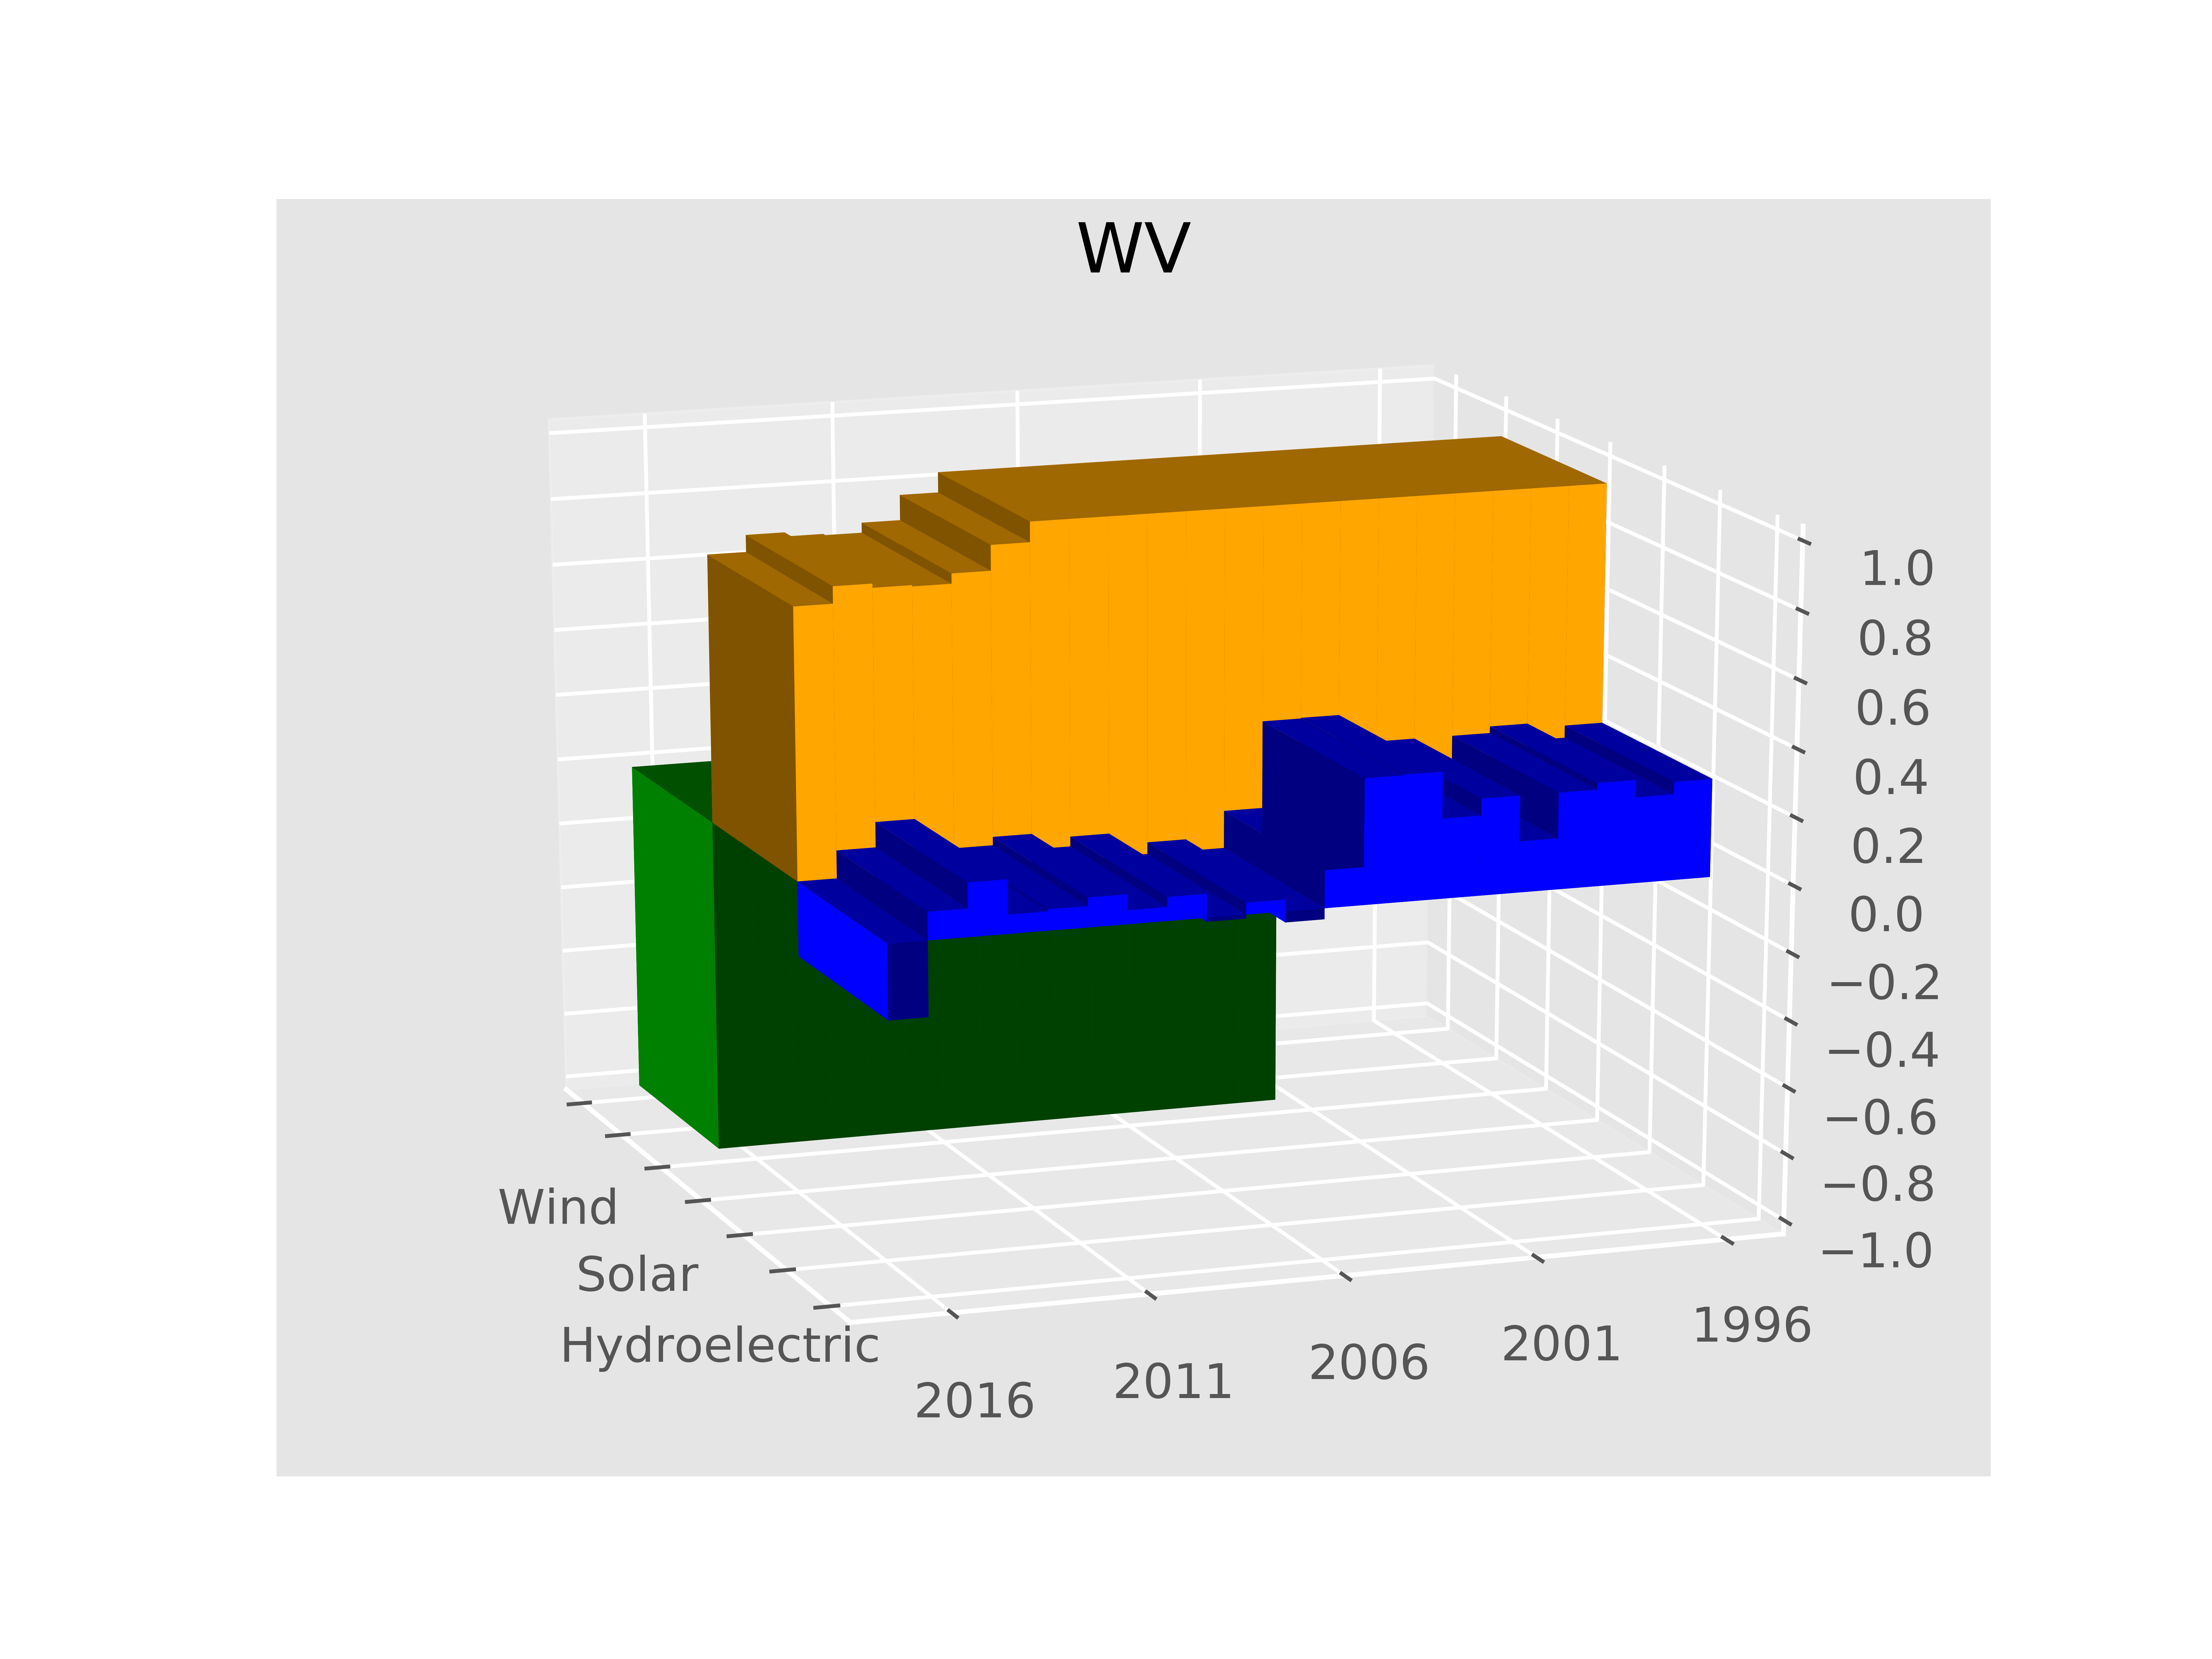
\includegraphics[width=0.85\textwidth]{WV.png}
\end{figure}

\newpage
Note: We used different orientations to show figures.

We also plotted the differences between generation and consumption of each renewable power source within each state, showing the trends of these differences over twenty years from 1996 to 2016. 

In terms of the analytical process, we aimed to map, for each state in the United States, the trends of the \textit{market potential} of each of the three renewable energy sources of interest (hydroelectric, solar, and wind) through the progression of the past two decades. As a result, our analysis required a suitable and statistically-accurate definition of \textit{market potential}. By weighing various factors of the information given through the data sets, particularly that presented in \textit{seds.csv}, we evaluated potential $U_M$ as a function of energy production ($P$) and raw consumption ($C$) as follows:
\[
  U_M(P, C) =
  \begin{cases}
    0 & \text{if $P,C=0$} \\
    -1 & \text{if $C=0$ and $P\neq0$} \\
    -1 & \text{if $\dfrac{P}{C}>2$} \\
    1-\dfrac{P}{C} & \text{otherwise} \\
  \end{cases}
\]
Consequently, using this piecewise definition of $U_M$, we were able to normalize and bound the data for the three renewable energy types, locking values between $-1$ and 1, inclusive. We ran into several issues when simply and naively implementing a $1-\dfrac{P}{C}$ definition, such as how to represent an accurate market potential for states with zero consumption, as well as possibly zero production. Gauging these edge cases and extreme factors, we deemed the above piecewise definition competent and justifiable, resulting in a precise model that generates a potential gradient, with $-1$ being of the lowest market potential, and $1$ being of the highest market potential, both inclusive bounds.

From this data, we see that some states have recently begun to increase generation of renewable energy, especially in solar power plants. This may be a result of furthered technology in solar panel technology as well as decreased prices for their materials, indicating that the solar energy market will likely rise within the next few decades. 
\newpage

\section{Conclusion}
From our analyses, we show that based on generation and consumption of solar, hydroelectric, and wind energy, the coastal regions, along with midwest states, have large market potential for investment in terms of renewable energy.

For future considerations and further analysis with the given data for our topic question, we hope to be able to incorporate more statistical and data-centered factors in our evaluation of market potential, including but not limited to values such as consumption per capita, population growth rate, education of renewable energies prevalence, and available land space with its accompanying cost. Moreover, we would attempt to build a predictive regression model for each of the states, generating and predicting trends in market potential values in the next 20 years based on our data and models. In order to do so, we would have to test various regression models, such as logarithmic or polynomial, finding the one that would best match trends in a particular state, or even a certain region. As of now, a logistic regression test would be of the brightest outlook, and we hope to extend our analysis as such in the future.
\end{document}